\section{Theoretical Analysis}
\label{sec:analysis}

\par In this section, we will analyse our theoretical model of the audio amplifier circuit in terms of the voltage gain, input and output impedances, and band width. The audio amplifier, as explained in the introduction is composed by two stages: the gain stage and the output stage. The first one provides a high gain and input impedance, however, it cames with a high output impedance that could degrade the signal transmitted to the load (by voltage division), which is not desirable. Thats why we need the second stage, which has a small gain ($\approx 1$), but provides also a small output impedance. Combining the two circuits, one can obtain a stable audio amplifier with good gain.
 
\subsection{Gain stage}
\label{subsec:gain_stage}

%Incluir imagem do primeiro circuito sem o thévenin aplicado com os dois condensadores

\par We will start by explaining why we need the components in the gain stage:

\begin{itemize}
\item The resistor $R_{C1}$, connected to the collector terminal of the transistor, is important to obtain a high gain as we will se in the operating point analysis.
\item The resistor $R_{E1}$, connected to the emmiter terminal of the transistor, ensures a temperature stabilization effect by imposing a negative feedback loop. That is important because some paramaters of the transistor are temperature dependent.
\item As we will see next, having the resistor $R_{E1}$ is not good for the AC gain. So, using the capacitor $C_b$ in parallel with the resistor we can make a short circuit for medium frequencies of $v_{IN}$, and the effect of the resistor can be neglected for the incremental analysis (because it is in parallel with a short circuit). For the operating point (DC), there is no AC component and the capacitor behaves like a open circuit, therefore, the resistor have the function of stabilization.
\item Because $v_{IN}$ has no DC component, we need a bias circuit, composed by the voltage supplier $V_{CC}$ and two resitors $R_{B1}$ and $R_{B2}$, that ensures the transistor is in the forward active region (FAR), where $V_{CE}>V_{BEON}$. We can simplify this circuit to a Thévenin's equivalent as showed in the next image. 
\item Also, we need another capacitor $C_i$ to block the $0V$ DC component of $v_{IN}$, creating an open circuit for low frequencies (DC analysis). Otherwise, the transistor wouldn't be in FAR. 
\end{itemize}

\subsubsection{Operating point for gain stage}
\label{subsec:OP1}

\par With the simplifications of the capacitors made before for low frequencies and without the voltage $v_{IN}$ (which only has AC component), we can write the following circuit to make the operating point analysis:

%Introduzir imagem do OP1 com thévenin
\begin{figure}[H] \centering
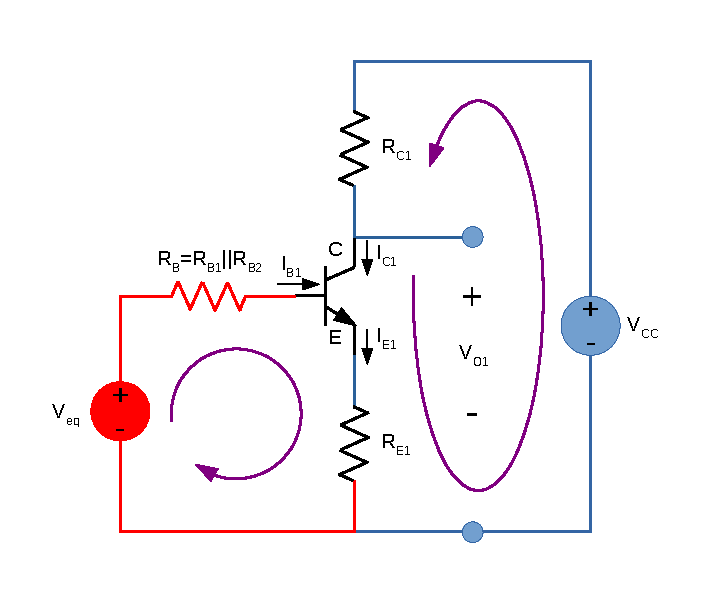
\includegraphics[width=0.8 \linewidth]{gain_stage.eps}
\caption{Gain stage circuit simplified to operating point.}
\label{fig:gain_stage}
\end{figure}

\par First we reduce the bias circuit to a Thévenin's equivalent obtaining the resistor $R_B$ and the equivalent voltage $V_{eq}$:

\begin{equation}
R_B=R_{B1}||R_{B2}=\frac{R_{B1}R_{B2}}{R_{B1}+R_{B2}
\end{equation}
\begin{equation}
V_{eq}=\frac{R_{B2}}{R_{B1}+R_{B2}V_{CC}
\end{equation}

\par Then we can write KVL to the left mesh, where $V_{BEON}\approx0.7$:
\begin{equation}
-V_{eq}+R_BI_B+V_{BEON}+R_{E1}I_{E1}=0
\end{equation}
\par The currents in the NPN transistor are related by the parameter $\beta _{FN}=178.7$ accordingly to the following equations:
\begin{equation}
I_{E1}=(1+\beta _{FN})I_{B1}
\end{equation}
\begin{equation}
I_{C1}=\beta _{FN}I_{B1}
\end{equation}

\par With the previous equations, we can write a equation to obtain $I_B$ and then, all the other currents in the transistor:
\begin{equation}
I_{B1}=\frac{V_{eq}-V_{ON}}{R_{B1}+(1+\beta _F)R_{E1}}
\end{equation}

\par After that, it's easy to compute the other DC voltages:

\begin{equation}
V_{O1}=V_{CC}-R_{C1}I_{C1}
\end{equation}
\begin{equation}
V_{E1}=R_{E1}I_{E1}
\end{equation}
\begin{equation}
V_{CE}=V_{O1}-V_{E1}
\end{equation}
\par To ensure that the transistor is in the FAR, the next condition must be verified: $V_{CE}>V_{BEON}$. As we can see in the next table with the operating point values this was ensured.

%Por tabela com os valores de OP1
\begin{table}[H]
    \centering
    \begin{tabular}{|l|r|}
    \hline    
    {\bf Name} & {\bf Value} \\ \hline
    \input{../mat/op1.tex}
    \end{tabular}
     \caption{Some currents (A) and voltages (dB) from the operating point of gain stage.}
    \label{tab:op1}
  \end{table}

\par Comparing this values with the ones in the simulation section, we can see that the DC values are much bigger in the simulation then the ones we got in theoretical calculations. This is a simple model with many simplifications that could justify that errors. For instance, we assume that the capacitors are either a short circuit or a open circuit; we fixed the value of $V_{BEON}$ which depends of the values of the voltages in the rest of the circuit; we used a simple model for AC calculations, using only resistors and dependent current sources (the reality is much more complicated); the ngspice model is much more complex and has a lot of parameters not included in our model. 


\subsubsection{Incremental analysis for gain stage}
\label{subsec:inc1}

\par Now, with the values of the operating point we can make the incremental analysis, for medium frequencies. As explained before, with this frequencies the capacitor $C_b$ is an open circuit, therefore, we can use the following incremental model (without the resistor $R_{E1}$):

%Imagem incr1
\begin{figure}[H] \centering
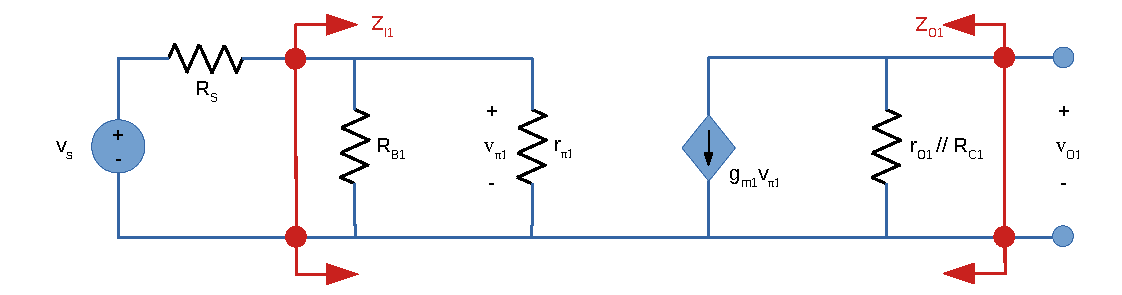
\includegraphics[width=0.8 \linewidth]{incremental1.eps}
\caption{Incremental model circuit for gain stage.}
\label{fig:inc1}
\end{figure}

\par The incremental parameters for this NPN transistor are given by:

\begin{equation}
gm1=\frac{I_{C1}}{V_T}
\end{equation}
\begin{equation}
r_{\pi 1}=\frac{\beta _{FN}}{g_{m1}}
\end{equation}
\begin{equation}
r_{o1}=\frac{V_{AFN}}{I_{C1}}
\end{equation}

\par With $V_{AFN}=69.7V$ and $V_T=25e^{-3}V$. Now we can compute the gain of the gain stage given by:

\begin{equation}
A_{V1}=\frac{R_{SB}}{R_S}R_{C1}\frac{-g_{m1}r_{\pi 1}r_{o1}}{(r_{o1}+R_{C1})(R_{SB}+r_{\pi 1})}
\end{equation}
\par With $R_{SB}=\frac {R_BR_S}{R_B+R_S}$

\par To compute the impedances of the gain stage we must consider again the resistor $R_{E1}$ between ground and emitter (not represented in the figure). To compute the output impedance we must also put $v_S=0$, making a short circuit. The input and output impedances are given, respectively, by:

\begin{equation}
Z_{I1}=\frac{1}{\frac{1}{R_B}+\frac{1}{\frac{(r_{o1}+R_{C1}+R_{E1})*(r_{\pi 1}+R_{E1})+g_{m1}*R_{E1}*r_{o1}*r_{\pi 1} - R_{E1}^2)}{r_{o1}+R_{C1}+R_{E1}}}}
\end{equation} 
\begin{equation}
Z_{O1} = \frac{1}{\frac{1}{Z_X}+\frac{1}{R_{C1}}}
\end{equation}
\par Where $Z_X$ is given by:
\begin{equation}
Z_X = r_{o1}*\frac{R_{SB}+\frac{r_{\pi 1}*R_{E1}}{RSB+rpi1+RE1}}{\frac{1}{\frac{1}{r_{o1}}+\frac{1}{rpi1+RSB}+\frac{1}{RE1}+\frac{gm1*rpi1}{rpi1+RSB}}}
\end{equation}

\par In the next table we print the theoretical results of the impedances and gain for the gain stage:

 %tabela impedancias e gain do gain stage
 \begin{table}[H]
    \centering
    \begin{tabular}{|l|r|}
    \hline    
    {\bf Name} & {\bf Value} \\ \hline
    \input{../mat/imp_gain1.tex}
    \end{tabular}
     \caption{Impedances and gain (dB) for gain stage.}
    \label{tab:inc1}
  \end{table}
 
 \par As we can see, the output impedance is still very high, which is not desirable. However this is desirable for the input impedance, which has already a good value to ensure that the input voltage isn't being degraded by the resistor $R_S$. The gain obtained is also good. Notice that this stage is an inverting amplifier, and the gain (in volts) is negative.
 
\subsubsection{Incremental analysis for output stage}
\label{subsec:op2}

 \begin{figure}[H] \centering
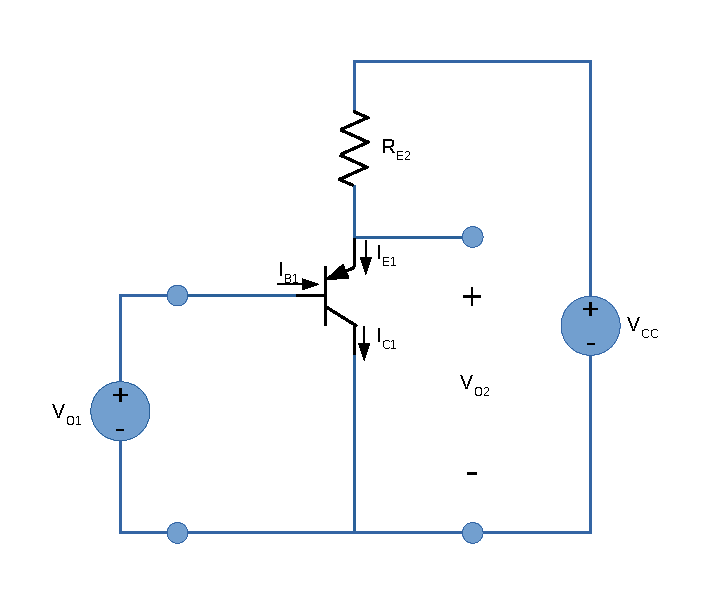
\includegraphics[width=0.8 \linewidth]{output_stage.eps}
\caption{Output stage circuit simplified to operating point.}
\label{fig:output_stage}
\end{figure}
 
 
 \par The output stage is similar to the gain stage, however it contains a PNP transistor with a higher value of the parameter $\beta _{FP}=227.3$ and it doesn't have the bias circuit. The other parameters are given by $V_{AFP}=37.2V$, $V_{EBON}=0.7$. The main goal of this sub circuit is to achieve a small output impedance.
 
\subsubsection{Operating point for the output stage}

\par The calculations for this operating point follow the same logic of the ones derived in subsection \ref{subsec:OP1}. With KCL equations one can derive the following expression.

\begin{equation}
I_{E2}=\frac{V_{CC}-V_{EBON}-V_{O1}}{R_{E2}}
\end{equation}
 
\par Then we can obtain the other currents in the transistors with the same raletions utilized in subsection \ref{subsec:OP1}. Notice that the output voltage of the first stage $V_{O1}$ is now the input voltage of this stage.
\par Now we can obtain $V_{O2}$, the output DC voltage of the total circuit:

\begin{equation}
V_{O2}=V_{CC}- R_{E2}I_{E2}
\end{equation} 
 
 \par The next table show the theoretical results for this operating point.
 
 %tabela OP2
 \begin{table}[H]
    \centering
    \begin{tabular}{|l|r|}
    \hline    
    {\bf Name} & {\bf Value} \\ \hline
    \input{../mat/op2.tex}
    \end{tabular}
     \caption{Some currents (A) and voltages (dB) from the operating point of output stage.}
    \label{tab:op2}
  \end{table}
 
 \subsubsection{Incremental analysis for the output stage}
 
 %imagem inc2
 \begin{figure}[H] \centering
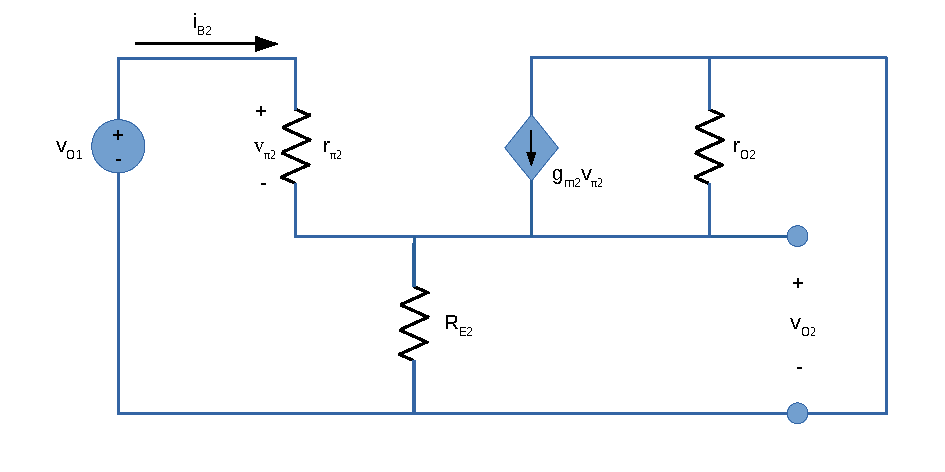
\includegraphics[width=0.8 \linewidth]{incremental2.eps}
\caption{Incremental model circuit for output stage.}
\label{fig:incremental2}
\end{figure}
 
 \par To make the incremental analysis we use the model in the image before. Using KCL in the transistor node, one can obtain this equation for gain:
 
 \begin{equation}
 A_{V2} = \frac{g_{m2}}{g_{m2}+g_{\pi 2}+g_{o2}+g_{e2}}
 \end{equation}
 
 \par Where $g_{\pi 2}=\frac{1}{r_{\pi 2}}$, $g_{o2}=\frac{1}{r_{o2}}$ and $g_{e2}=\frac{1}{R_{E2}}$ are the condutancies.
 
 \par Following the same logic of subsection \label{subsec:inc1}, the input and output impedances for output stage are given by:
 
 \begin{equation}
 Z_{I1}= \frac{g_{m2}+g_{\pi 2}+g_{o2}+g_{e2}}{g_{\pi 2}(g_{\pi 2}+g_{o2}+g_{e2}}
 \end{equation}
  \begin{equation}
 Z_{O1} = \frac{1}{g_{m2}+g_{\pi 2}+g_{o2}+g_{e2}}
 \end{equation}
 
 \par The results obtained are printed in the next table:
 
%tab inc2
 \begin{table}[H]
    \centering
    \begin{tabular}{|l|r|}
    \hline    
    {\bf Name} & {\bf Value} \\ \hline
    \input{../mat/imp_gain2.tex}
    \end{tabular}
     \caption{Impedances and gain (dB) for output stage.}
    \label{tab:inc2}
  \end{table}

\par As we can see, the output impedance of this circuit is surprisingly small, which was our goal. The gain is $\approx 1$, that means this circuit doesn't reduce much the voltage gain obtained in the first stage.

\par It's important to check if the two stages are compatible in terms of input and output impedances, to ensure that there are no significant losses in signal between stages. Because the output impedance of the gain stage $Z_{O1}$ is much smaller than the input impedance of the second stage $Z_{I1}$ (by more than a factor of 10), the voltage will be effectively transmited from the first stage to the second one, without many losses.

\subsection{Total gain and impedances}

\par Finally, we will calculate the total impedances and gain, in incremental terms. To achieve this, we can write the incremental model to the whole circuit, simplify the gain stage to a dependent voltage source and his impedances, and finally aplying KCL equation to the PNP transistor node. To compute the total output impedance $Z_O$ we shut off input voltage and, therefore, the circuit becomes much simpler. The total input impedance is equal to $Z_{I1}$.

\begin{equation}
g_B = \frac{1}{\frac{1}{g_{\pi 2}}+Z_{O1}}
\end{equation}
\begin{equation}
A_V = \frac{\frac{g_B+g_{m2}}{g_{\pi 2}g_B}}{\frac{g_B+g_{e2}+g_{O2}+g_{m2}}{g_{\pi 2}g_B}}A_{V1}
\end{equation}
\begin{equation}
Z_I=Z_{I1}
\end{equation}
\begin{equation}
Z_O=\frac{1}{g_{o2}+\frac{g_{m2}g_B}{g_{\pi 2}+g_{e2}+g_B}}
\end{equation}

%incluir tabela total
 \begin{table}[H]
    \centering
    \begin{tabular}{|l|r|}
    \hline    
    {\bf Name} & {\bf Value} \\ \hline
    \input{../mat/imp_gaintot.tex}
    \end{tabular}
     \caption{Total impedances and gain (dB).}
    \label{tab:tot}
  \end{table}

\par The theoretical value of $Z_O$ is similar to the one obtained in the simulation and is very low, as we wanted. This is important when we connect a load with small impedance (like the speaker) to the amplifier. $Z_I$ and the gain $A_V$ are big values, as we wanted. Althought they are in the same order of magnitude as the values obtained in the simulation, the errors are still very large, due to the aproximations that this simple theoretical model does.

\par Although we obtained a constant value of gain in the theoretical calculations, regardless of the frequency of the signal, this is not the real scenario. As we saw on the simulation analysis, there is a lower and upper cut-off frequencies, where the gain starts droping. In this theoretical model we assumed medium frequencies and simplified the capacitors to short circuits or open circuits. To obtain more realistic results we should analyse the entire circuit with node or mesh incremental analysis, replacing the capacitors with his impedances. We are no doing that here, but we can observe the cut-off frequencies in the simulation chapter. 

